\subsection{Histogram equalization}

\begin{center}
	\textit{''... is a method in image processing of contrast adjustment using the image's histogram.''}
\end{center}

\subsubsection{Fordele}

Et histogram beskriver intensitets-niveauerne i et billedet. Ved at ''udligne'' histogrammet kan man opnå en række fordele:

\begin{itemize}
	\item Bedre få vist benstruktur i et røntgenbillede.
	\item Trække flere detaljer ud i et over- eller undereksponeret billede.
\end{itemize}

Denne funktion er invertible, altså hvis vi kender \textit{histogram equalization function}'en kan vi genskabe det originale billede.

Figur~\ref{fig:histogram-eq} viser enkelt hvad der menes med udligning.

\begin{figure}[H]
	\centering
	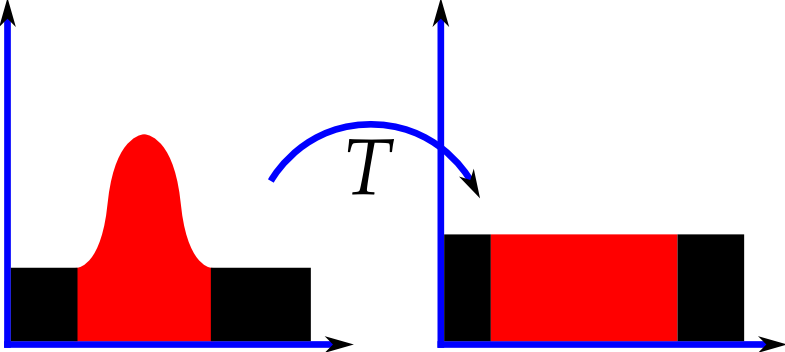
\includegraphics[width=0.6\linewidth]{figs/spm01/histogram-eq.png}
	\caption{Histogram equalization.}
	\label{fig:histogram-eq}
\end{figure}

\subsubsection{Ulemper}
Det er ikke uden pris at vi kan lave denne udligning. Vi mister nogle ting:

\begin{itemize}
	\item Metoden kan forøge baggrundsstøj og derved minske det brugbare signal.
	\item Kan skabe en synlig gradient, se Figur~\ref{fig:gradient}.
\end{itemize}

\begin{figure}[H]
	\centering
	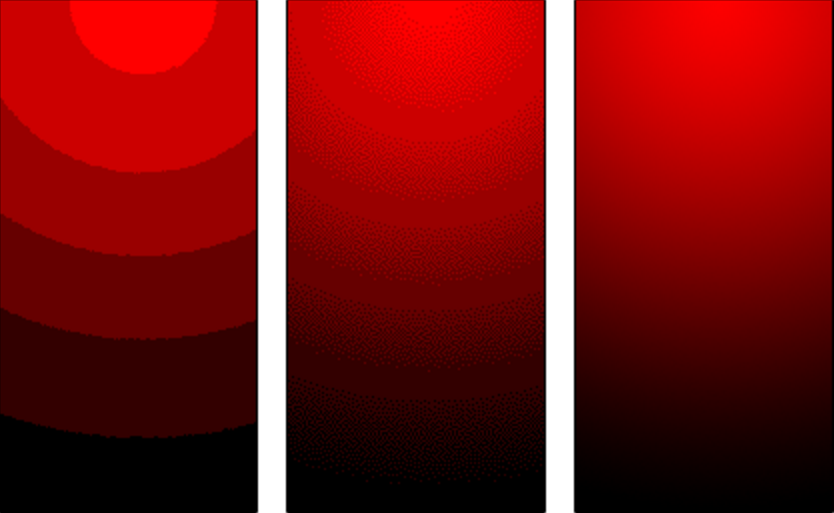
\includegraphics[width=0.7\linewidth]{figs/spm01/gradient}
	\caption{Fra venstre: 8-bit, 8-bit dithered og 24-bit gradient.}
	\label{fig:gradient}
\end{figure}
